\section{نکات پیاده‌سازی پروژه}

پیاده‌سازی پروژه در زبان جاوا انجام گرفت. یکی از نکات مهم و قابل توجه در پیاده‌سازی این پروژه این است که تمام مراحل انجام کار  به طور کاملاً خودکار انجام شود و در هیچ مرحله‌ای نیاز به دخالت عامل خارجی  ندارد بجز پیکربندی اولیه مانند آدرس پایگاه داده. همچنین در تمام مراحل سعی شده است که  اصول لازم در طراحی معماری نرم‌افزار به کار گرفته شود و نیازمندی‌های کیفی پروژه نیز مد نظر قرار گیرد. این نیازمندی‌ها شامل موارد زیر است:
\begin{enumerate}
\item 
\واژه{کارایی} : جهت پاسخ به این نیازمندی از پایگاه داده استفاده شده است.
\item
قابلیت نگهداری: این قابلیت از سایرین بیشتر حائز اهمیت است. زیرا پروژه‌های پروژهشی معمولا به صورت مستقیم کاربران عمومی ندارند و از این جهت نیازمند کارایی بالا یا رابط گرافیکی کاربر پسند نیستند. استفاده آن‌ها معمولاً در گسترش آن‌ها توسط سایر محققین است که راه را ادامه خواهند داد. 
\begin{itemize}
\item

 برای پاسخ به این نیازمندی اصول مربوط به کدنویسی  در فصل سوم و چهارم کتاب  \cite{martin2009clean} به کار گرفته شده است.
 \item
 از الگوهای نرم افزاری پرکاربرد مانند \نام{اداپتور}{Adaptor}،  \نام{فکتوری}{Factory} و \نام{سینگلتون}{Singelton} استفاده شده است.
 \item
 به منظور جلوگیری از قطعه کد تکراری از وراثت و توابع \واژه{عمومی} استفاده شده است. همینطور عمق وراثت از عدد ۳ بیشتر نشده است زیرا وراثت عمیق از خوانایی کد می‌کاهد و محل اشتباه خواهد بود. 
\end{itemize}
\item
امنیت: از آنجا که پروژه قرار نیست به استفاده‌ی عموم برسد و کاربران عمل متخاصمانه‌ای انجام نخواهند داد   به نوع خاصی از امنیت  نسبت به انواع متداول نیاز دارد.  باید روند توسعه‌ی پروژه دارای امنیت باشد. از این نظر که کدها مفقود نشوند یا در صورت اشتباه در توسعه بتوان پروژه را به حالت قبل بازگرداند. در این راستا کدهای پروژه در مخزن نرم‌افزاری از نوع گیت نگهداری شده که یک مخزن در کامپیوتر شخصی و دیگری در سایت \نام{بیت‌باکت}{Bitbucket - \url{https://bitbucket.org/alimohebbi/bug_predict }} 
قرار دارد. مزیت این سایت نسبت به گیت‌هاب این است مخازن خصوصی  را به صورت رایگان ارائه می دهد. در مخازن خصوصی  اجازه‌ی دسترسی تنها به  افراد تعیین شده از طرف مالک  داده می‌شود و عموم کاربران به آن دسترسی ندارند. از ابتدای شروع پیاده‌سازی کدها در مخازن بروزرسانی شده است. نمایی از ثبت‌های مختلف پروژه در مخزن در شکل \ref{fig:bitbucket}
آورده شده است. 
\end{enumerate}

 \begin{figure}[H]
	\centering
	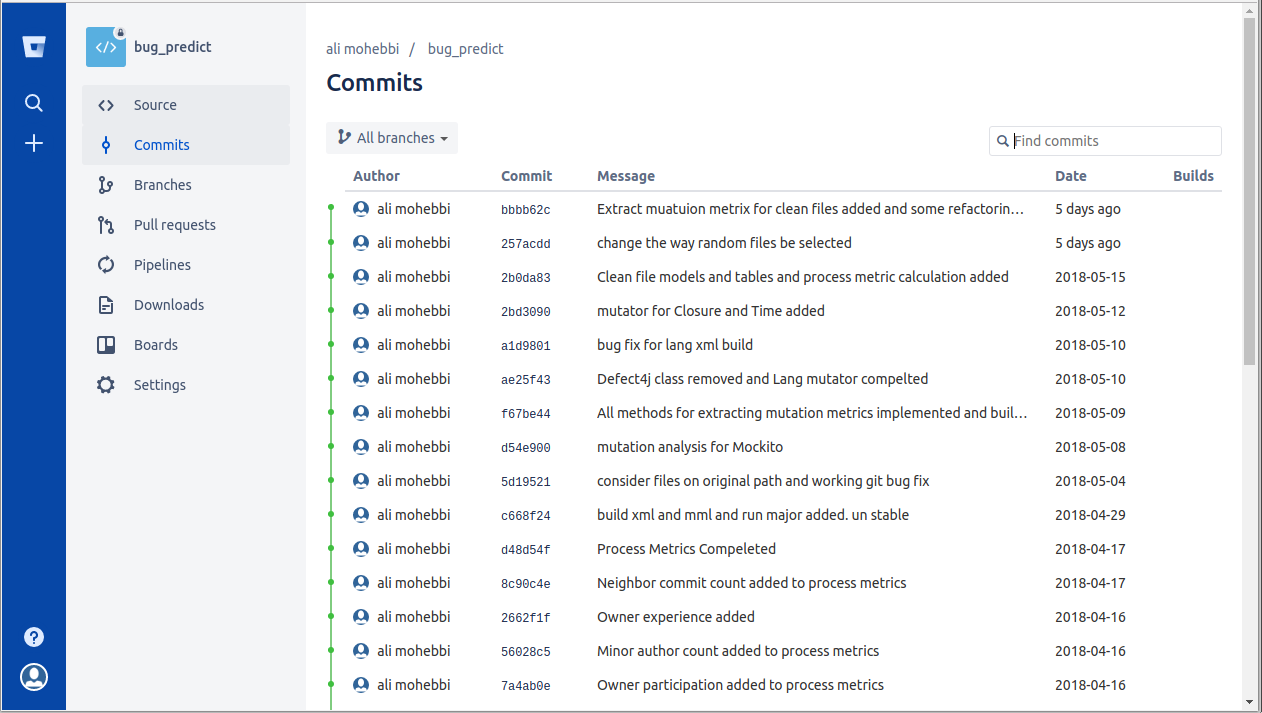
\includegraphics[width=1\textwidth]{img/case_study/bitbucket.png}
	\caption{نمایی از مخزن نرم‌افزاری}
	\label{fig:bitbucket}
\end{figure}



\section{استخراج اطلاعات و معیارها}
در این قسمت  چگونگی استخراج معیارهای رویکرد اول شرح داده می‌شود. ابتدا لازم است اطلاعات مربوط به ثبت‌های  حاوی خطا از ابزار \lr{defects4j} بازیابی شود و سپس این اطلاعات با استفاده از مخرن نرم‌افزاری تکمیل شود. در مراحل بعد معیار‌های فرآیند و سپس معیارهای جهش استخراج خواهند شد. 

\subsection{ استخراج اطلاعات مربوط به ثبت‌های   حاوی خطا}
اطلاعاتی که درباره‌ی ثبت‌های حاوی خطا قابل بازیابی است در زیر آمده است:
\begin{enumerate}
\item شناسه‌ی ثبت در مخزن 
\item نام پرونده‌ی حاوی خطا
\item شماره‌ی خطا در ابزار \lr{defects4j}
\item شماره‌ی ثبت تعمیر خطا
\item نام پروژه
\item نام انتشار قبلی پروژه
\item شماره‌ی ثبت انتشار قبلی پروژه
\end{enumerate}

از میان اطلاعات بالا همگی به سادگی با استفاده از ابزار \lr{defect4j} قابل استخراج است بجز دو مورد آخر. همچنین شماره‌ی ثبت تعمیر مورد استفاده قرار نگرفت ولی نگهداری شد چراکه ممکن است در پژوهش‌های دیگر لازم شود. 
برای بدست آوردن اطلاعات مربوط به هر انتشار لازم است که مخرن نرم‌افزاری هر پروژه مورد بررسی قرار گیرد. در  مخازن پروژه‌های نرم‌افزاری  از نوع گیت برای مشخص کردن یک رویداد مهم از \نام{تگ}{Tag} استفاده می‌شود. هر تگ می‌تواند به یک ثبت از برنامه اشاره کند. تگ می‌تواند نمایانگر رویدادهایی چون انتشار برنامه، انتشار بتا، و یا کاندید انتشار باشد. بنابرین با استفاده از تگ می‌تواند انتشار را پیدا کرد.\\

تگ‌های مخازن گیت دو نوع \واژه{سبک‌وزن} و \واژه{حاشیه‌نویسی شده}  دارد که در میان پروژه‌های مورد مطالعه از هر دو نوع جهت مشخص کردن انتشار استفاده شده است.  کار کردن با این دو نوع تگ دارای تفاوت‌هایی در پیاده‌سازی است که در اینجا از پرداختن به جزییات صرف نظر می‌شود. \\ ابتدا همه‌ی تگ‌های موجود در مخازن نرم‌افزاری استخراج می‌شود و در پایگاه داده قرار می‌گیرد. از میان تگ‌های استخراج شده تگ‌های نامرتبط با انتشار از پایگاه داده حذف می‌شود. تگ‌های نامرتبط با توجه به نام آنها مشخص می‌شود به عنوان مثال تگ‌هایی که حاوی لغات Beta یا Dev هستند نامرتبط  محسوب می‌شوند. در نهایت جدولی به نام ReleaseProject ساخته می‌شود که در آن اطلاعات انتشارهای مختلف وجود دارد. نمایی از این جدول در شکل \ref{fig:project-release} آمده است. \\
\begin{figure}[H]
	\centering
	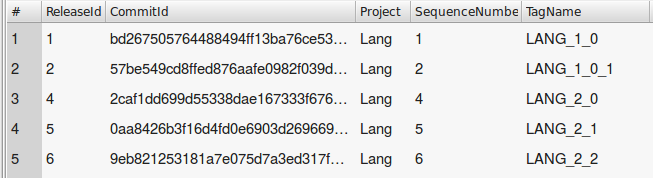
\includegraphics[width=1\textwidth]{img/case_study/project-release.png}
	\caption{نمایی از جدول محتوای انتشارها}
	\label{fig:project-release}
\end{figure}


در قدم بعدی باید مشخص شود اولین انتشار ماقبل هر ثبت حاوی خطا کدام است. برای این منظور لیست ثبت‌ها  در یک پروژه به ترتیب زمانی بررسی می‌شود. اولین ثبت  ماقبل ثبت مورد نظر که مربوط به یک انتشار است یافت می‌شود و به عنوان انتشار ماقبل آن ثبت در نظر گرفته می‌شود. \\

 در نهایت جدولی به نام BugInfo تولید شده که نمایی از آن در شکل \ref{fig:bug-info} آمده است. این جدول ۴۰۵ سطر دارد که بیشتر از تعداد کل خطاهای ذکر شده در مجموعه داده‌ی \lr{defects4j} است. علت این است که یک خطا می‌تواند خطا در چندین پرونده به طور همزمان باشد و از آنجا که پیش‌بینی در سطح پرونده انجام می‌شود لازم است اطلاعات برای پرونده‌ها ذخیره شود.

\begin{figure}[H]
\centering
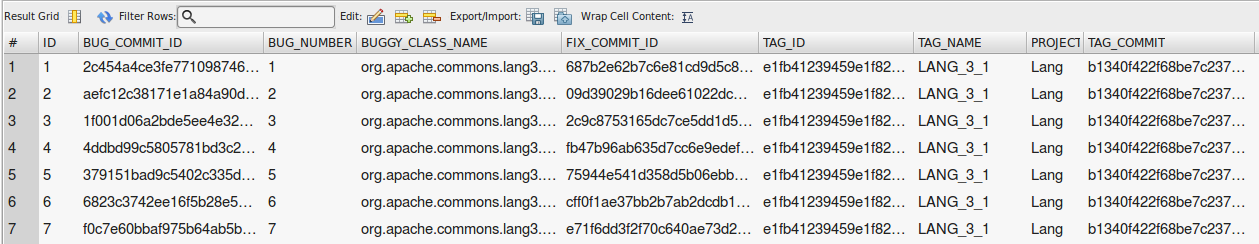
\includegraphics[width=1\textwidth]{img/case_study/bug-info.png}
\caption{نمایی از جدول محتوای اطلاعات پرونده‌های حاوی خطا}
\label{fig:bug-info}
\end{figure}

\subsection{انتخاب پرونده‌های سالم}
همانطور که مطرح شد تعداد پرونده‌های حاوی خطا برابر ۴۰۵ عدد است که از تعداد کل پرونده‌ها کمتر است. بنابرین جهت ساخت مدل‌های بدون جهت‌گیری به همین تعداد پرونده‌های بدون خطا به طور تصادفی انتخاب می‌شود. بدین ترتیب یک مجموعه داده‌ی \واژه{متعادل} حاوی ۸۱۰ پرونده ساخته شده است. این روش طبق مقاله‌ی \cite{johannessen2008data} به کار گرفته شده است. در این انتخاب به تعداد پرونده‌های حاوی خطا، پرونده‌های بدون خطا انتخاب می‌شود. \\به ازای هر پرونده‌ی دارای خطا در همان ثبت از پروژه‌ی مربوط، یک پرونده‌ی بدون خطا به صورت تصادفی انتخاب می‌شود. برای این کار لیست تمام پرونده‌های داخل پروژه در ثبت پرونده حاوی خطا در نظر گرفته می‌شود و یک پرونده به صورت تصادفی انتخاب می‌شود. این پرونده نباید جز پرونده‌های حاوی خطا در آن ثبت از  پروژه باشد.   همانطور که گفته شد یک ثبت ممکن است بیش از یک پرونده حاوی خطا داشته باشد. همچنین ممکن  است این پرونده در ثبت‌های بعدی یا قبلی خطا داشته باشد و از این نظر محدودیتی ندارد. سپس مشخصات این پرونده در جدول CleanInfo قرار می گیرد. نمایی از این جدول در تصویر \ref{fig:clean-info} آورده شده است.
\begin{figure}[H]
	\centering
	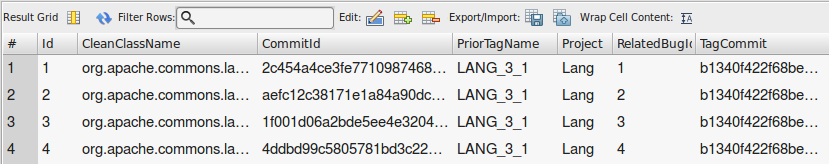
\includegraphics[width=1\textwidth]{img/case_study/clean-info.png}
	\caption{نمایی از جدول محتوای اطلاعات پرونده‌های سالم}
	\label{fig:clean-info}
\end{figure}



\subsection{ استخراج معیارهای فرآیند}
در  این قسمت نحوه‌ی ساخت جداول مورد نیاز در استخراج معیارهای ذکر شده در قسمت \ref{sec:method-phase1} بیان می‌شود. \\
\textbf{جداول اطلاعات ثبت‌ها و پرونده‌های تغییر یافته}


کل ثبت‌های پروژه‌ها مورد بررسی قرار گرفت و دو جدول تولید شد. جدول اول  CommitInfo‌    اطلاعات کلی ثبت‌ها را در بر می‌گیرد و جدول دوم  CommitChangedFile   اطلاعات مربوط به پرونده‌هایی که در یک ثبت از برنامه نسبت به ثبت قبلی تغییر کرده است نگهداری می‌شود.  در این جدول برای هر پرونده تعداد خطوط اضافه و کم شده نسبت به ثبت قبلی ذخیره شده است. در جدول اول \lr{Sequence\textunderscore Number} نشان می‌دهد که چندمین نسخه از ابتدای پروژه می‌باشد و این عدد در هنگام بررسی‌ها به آن ثبت داده‌ شده زیرا برای یافتن ثبت‌های بین ثبت کنونی و ثبت مربوط به انتشار قبلی لازم است از آنها استفاده شود. برای یافتن ثبت‌های بین انتشار و ثبت مورد نظر نمی‌توان از تاریخ ثبت آنها استفاده کرد. زیرا تعداد زیادی از ثبت‌های ابتدای  برخی پروژه‌های مورد مطالعه دارای تاریخ یکسانی هستند  بنابرین استفاده از تاریخ غیر ممکن می‌شود. علت داشتن تاریخ یکسان احتمالاً مهاجرت از یک نوع مخرن نرم‌افزاری به نوع گیت بوده است. \\
  هر سطر از جدول دوم یک کلید خارجی دارد به سطری از جدول اول. قسمتی از جدول CommitInfo  در شکل \ref{fig:commit-info} و جدول CommitChangeFile در شکل \ref{fig:change-file-info}  زیر آمده است:

\begin{figure}[H]
	\centering
	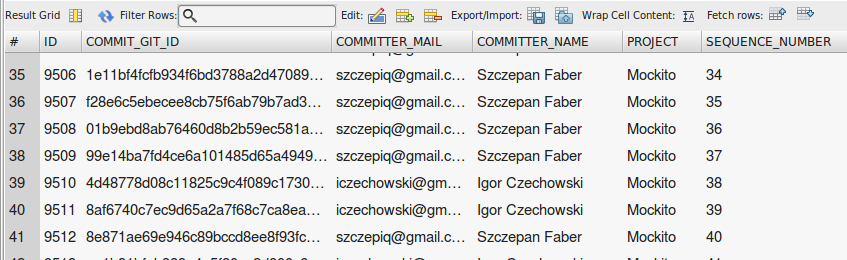
\includegraphics[width=1\textwidth]{img/case_study/commit-info.png}
	\caption{نمایی از جدول اطلاعات ثبت‌ها}
	\label{fig:commit-info}
\end{figure}


\begin{figure}[H]
	\centering
	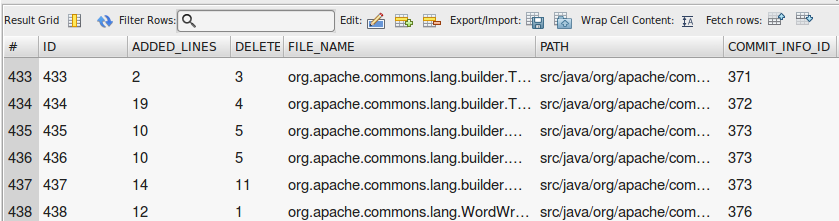
\includegraphics[width=1\textwidth]{img/case_study/change-file-info.png}
	\caption{ نمایی از جدول تغییرات پرونده‌ها در ثبت‌ها }
	\label{fig:change-file-info}
\end{figure}

\begin{comment}

در نهایت با استفاده از قطعه کد \ref{code:commit-info} اطلاعات مربوط به ثبت مورد نظر و ثبت انتشار بازیابی می‌شوند و سپس  از شماره‌ی دنباله‌ی آنها در پرسمان موجود در قطعه کد \ref{code:comm} استفاده می‌شود و معیار محاسبه می‌گردد.



\begin{latin}
	\begin{lstlisting}[language=SQL]
SELECT  * from CommitInfo CI where CI.COMMIT_GIT_ID = :gitId AND CI.PROJECT = :project
\end{lstlisting}
\end{latin}
\captionof{lstlisting}{بازیابی اطلاعات ثبت}
\label{code:commit-info}

\begin{latin}
\begin{lstlisting}[language=SQL]
SELECT  count(*) from CommitChangedFile CCzzz where CC.COMMIT_INFO_ID IN
	(SELECT CI.ID from CommitInfo CI WHERE CI.SEQUENCE_NUMBER BETWEEN 
	 :startSeq AND :endSeq AND CI.PROJECT = :project)
AND CC.FILE_NAME = :fileName
\end{lstlisting}
\end{latin}
\captionof{lstlisting}{محاسبه‌ی معیار تعداد ثبت‌ در سیستم کنترل نسخه}
\label{code:comm}

\متن‌سیاه{‫تعداد توسعه‌دهندگان فعال:‬}
به منظور محاسبه‌ی این معیار تعداد آدرس ایمیل‌های ثبت‌کننده‌های ثبت‌هایی شمرده می‌شود که آن ثبت‌ها شماره‌ی دنباله‌ی آنها بین شماره‌ی دنباله‌ی ثبت پرونده‌ی مورد نظر و ثبت انتشار قبلی است و همچنین پرونده‌ی مورد نظر در آن ثبت‌ها تغییر کرده است. به عبارت دیگر ثبت‌هایی که نام پرونده در جدول  CommitChangeFile  برای آن‌ها وجود دارد. 

\begin{latin}
\begin{lstlisting}[language=SQL]
SELECT  count(DISTINCT CI.COMMITTER_MAIL) from CommitInfo CI WHERE
CI.SEQUENCE_NUMBER BETWEEN :startSeq AND :endSeq AND CI.PROJECT = 
project AND CI.ID IN 
	(SELECT CC.COMMIT_INFO_ID from CommitChangedFile CC where CC.FILE_NAME = :fileName)
\end{lstlisting}
\end{latin}
\captionof{lstlisting}{محاسبه‌ی تعداد توسعه‌دهندگان فعال}

\textbf{تعداد توسعه‌دهندگان متمایز:}
برای محاسبه‌ی معیار از پرسمان قبلی استفاده می‌شود اما اینبار به جای استفاده \lr{Sequence\_Number} انتشار قبلی، عدد یک  قرار داده می‌شود که از ابتدای پروژه تعداد توسعه‌دهندگان شمرده شوند. 
\\

\متن‌سیاه{‫مقدار نرمال‌سازی شده‌ی تعداد خطوط اضافه شده:‬}
از پرسمان \ref{code:added-line-file} جهت محاسبه‌ی مجموع تعداد خطوط اضافه شده به پرونده در طول انتشار استفاده می‌شود و از پرسمان \ref{code:added-line-project} جهت محاسبه‌ی مجموع خطوط اضافه شده به پروژه استفاده می‌شود. سرانجام حاصل پرسمان اول بر دوم تقسیم می‌شود. 

\begin{latin}
	\begin{lstlisting}[language=SQL]
SELECT sum(CC.ADDED_LINES) from CommitChangedFile CC where
CC.COMMIT_INFO_ID IN
	(SELECT CI.ID from CommitInfo CI WHERE CI.SEQUENCE_NUMBER BETWEEN 
	:startSeq AND :endSeq AND CI.PROJECT = :project)
AND CC.FILE_NAME = :fileName
	\end{lstlisting}
\end{latin}
\captionof{lstlisting}{محاسبه‌ی تعداد خطوط اضافه شده به پرونده}
\label{code:added-line-file}

\begin{latin}
\begin{lstlisting}[language=SQL]
SELECT  sum(CC.ADDED_LINES) from CommitChangedFile CC where 
CC.COMMIT_INFO_ID IN
	(SELECT CI.ID from CommitInfo CI WHERE CI.SEQUENCE_NUMBER
	 BETWEEN :startSeq AND :endSeq AND CI.PROJECT = :project)
\end{lstlisting}
\end{latin}
\captionof{lstlisting}{محاسبه‌ی تعداد خطوط اضافه شده به پروژه}
\label{code:added-line-project}

\متن‌سیاه{‫مقدار نرمال‌سازی شده‌ی تعداد خطوط حذف شده:‬} به طور مشابه معیار قبلی محاسبه می‌گردد.
\end{comment}

\textbf{جدول مشارکت‌کنندگان:}
دستور Blame در Jgit نشان می‌دهد که هر خط از پرونده در یک ثبت  در کدام یک از ثبت‌های گذشته اضافه شده است.  با یافتن ثبت مسئول اضافه کردن آن خط نویسنده‌ی آن خط مشخص می‌شود که همان ثبت‌کننده است. با کمک این دستور به دلایل مشابه ساخت جداول مربوط به ثبت‌ها، جدولی با عنوان Participation ساخته شده که در آن هر سطر نشان می‌دهد که یک نویسنده در یک نسخه از برنامه چند درصد از خطوط به وی اختصاص دارد. در شکل \ref{fig:participation} نمایی از این جدول آورده شده است.  از این جدول علاوه بر محاسبه‌ی این معیار برای یافت سایر معیارها نیز استفاده خواهد شد. 

\begin{figure}[H]
	\centering
	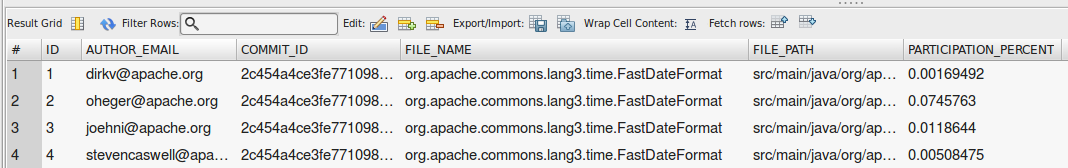
\includegraphics[width=1\textwidth]{img/case_study/participation.png}
	\caption{نمایی از جدول مشارکت‌کنندگان در ویرایش پرونده‌ها}
	\label{fig:participation}
\end{figure}

\begin{comment}

\begin{latin}
	\begin{lstlisting}[language=SQL]
SELECT max(PARTICIPATION_PERCENT) from Participation P 
where COMMIT_ID = :commitId AND FILE_NAME = :fileName")
\end{lstlisting}
\end{latin}
\captionof{lstlisting}{محاسبه‌ی درصد خطوط مالک پرونده}
\label{code:own}

\textbf{تعداد مشارکت‌کنندگان جزئی:‬}
 با استفاده از جدول Participation و پرسمان  \ref{code:minor}  معیار محاسبه می‌شود. مقدار minorThereshold برابر ۵ درصد قرار می‌گیرد.

\begin{latin}
	\begin{lstlisting}[language=SQL]
SELECT count(AUTHOR_EMAIL) from Participation P 
where COMMIT_ID = :commitId AND FILE_NAME = :fileName
and PARTICIPATION_PERCENT < :minorThreshold
\end{lstlisting}
\end{latin}
\captionof{lstlisting}{محاسبه‌ی تعداد مشارکت‌کنندگان جزئی}
\label{code:minor}

\textbf{تعداد ثبت‌های همسایگان:‬}
ابتدا لازم است که همسایگان پرونده در یک ثبت و نیز تعداد دفعات همسایگی در طول انتشار مشخص شود. این عمل به وسیله‌ی پرسمان \ref{code:neighbor} انجام می‌شود. سپس معیار تعداد ثبت‌ها در سیستم کنترل نسخه مشابه قبل با استفاده از کد \ref{code:comm} محاسبه می‌گردد و از آنها میانگین وزن‌دهی شده گرفته می‌شود.

\begin{latin}
\begin{lstlisting}[language=SQL]
SELECT FILE_NAME as `name`, count(ID) as `frequency` FROM
CommitChangedFile WHERE COMMIT_INFO_ID IN
	(SELECT COMMIT_INFO_ID FROM CommitChangedFile WHERE FILE_NAME = :fileName) 
AND COMMIT_INFO_ID IN
	(SELECT CI.ID from CommitInfo CI WHERE CI.SEQUENCE_NUMBER BETWEEN :startSeq AND :endSeq AND PROJECT = :project)
AND FILE_NAME != :fileName GROUP BY FILE_NAME
\end{lstlisting}
\end{latin}
\captionof{lstlisting}{یافتن همسایگان و تعدد همسایگی}
\label{code:neighbor}

\textbf{تعداد توسعه‌دهندگان فعال همسایگان:‬}
 به طور مشابه با معیار قبلی محاسبه می‌شود.\\
\textbf{‫تعداد توسعه‌دهندگان متمایز همسایگان:‬}
 به طور مشابه با معیار قبلی محاسبه می‌شود. \\

\textbf{تجربه‌ی مالک پرونده:‬‬}
 برای محاسبه‌ی معیار ابتدا   با استفاده از پرسمان \ref{code:find-owner} مالک پرونده مشخص می‌شود. سپس تعداد ثبت‌هایی که مالک پرونده از ابتدای پروژه تا آن زمان ثبت کرده است  با استفاده از پرسمان \ref{code:commit-of-commiter} شمرده می‌شود. به ترتیب از دو جدول Participation 
 و 
 CommitInfo  استفاده می‌شود.

\begin{latin}
\begin{lstlisting}[language=SQL]
SELECT AUTHOR_EMAIL FROM Participation P WHERE COMMIT_ID = :commitId 
AND FILE_NAME = :fileName AND PARTICIPATION_PERCENT  = 
	(SELECT max(PARTICIPATION_PERCENT) FROM Participation P2 
	 WHERE P2.COMMIT_ID = :commitId  AND P2.FILE_NAME = :fileName)
\end{lstlisting}
\end{latin}
\captionof{lstlisting}{یافتن مالک پرونده}
\label{code:find-owner}



\begin{latin}
\begin{lstlisting}[language=SQL]
SELECT  count(*) from CommitInfo CI where CI.SEQUENCE_NUMBER BETWEEN
:startSeq AND :endSeq AND CI.PROJECT = :project AND CI.COMMITTER_MAIL =
:authorEmail
\end{lstlisting}
\end{latin}
\captionof{lstlisting}{شمارش تعداد ثبت‌های یک ثبت کننده در بازه‌ی زمانی داده شده}
\label{code:commit-of-commiter}

\textbf{‫تجربه‌ی تمام مشارکت‌کنندگان:‬}
ابتدا همه‌ی توسعه‌دهندگان پرونده با استفاده از پرسمان \ref{code:contributers} مشخص می‌شوند.  سپس میزان تجربه‌ی هر یک با استفاده از پرسمان \ref{code:commit-of-commiter} جداگانه محاسبه می‌شود و از آن‌ها میانگین هندسی گرفته می شود. 
\begin{latin}
\begin{lstlisting}[language=SQL]
SELECT AUTHOR_EMAIL FROM Participation P WHERE COMMIT_ID = :commitId 
AND FILE_NAME = :fileName
\end{lstlisting}
\end{latin}
\captionof{lstlisting}{یافتن مشارکت‌کنندگان در پرونده}
\label{code:contributers}
\end{comment}

در نهایت جدولی برای معیارهای فرآیند تولید می‌شود که نمایی از آن در شکل \ref{fig:process-metics} آورده شده است. 
\begin{figure}[H]
	\centering
	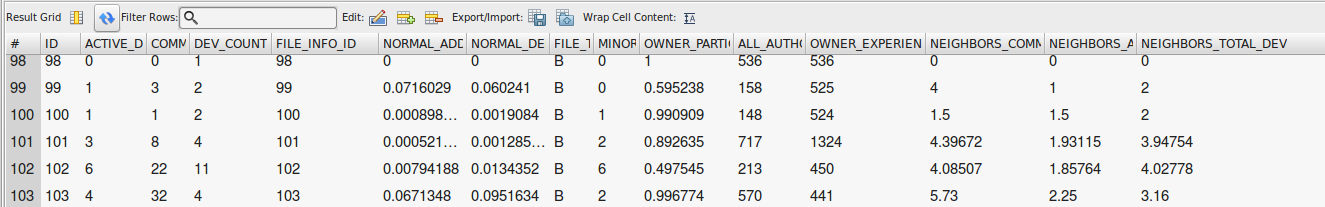
\includegraphics[width=1\textwidth]{img/case_study/process-metrics.png}
	\caption{نمایی از جدول معیارهای فرآیند }
	\label{fig:process-metics}
\end{figure}


\subsection{استخراج معیارهای جهش}
روند کلی به این صورت است که برای هر سطر از جدول BugInfo   یا CleanInfo که معادل یک  پرونده  در یک نسخه است ابتدا آن نسخه از برنامه در پوشه‌ی کاری قرار می‌گیرد. منظور از پوشه‌ی کاری محلی است  که پرونده‌های یک ثبت خاص از پروژه از مخزن نرم‌افزاری فراخوانی می‌شود و در آن قرار می گیرد. سپس به پرونده build.xml    و یا build.gradle  قطعه کدهایی  به منظور  اجرای  صحیح فرآیند ساخت اضافه می‌شود.  \\
همچنین جهت تولید جهش‌یافته و تحلیل جهش لازم است برای هر پروژه پیکربندی‌هایی انجام شود که این پیکربندی‌ها با اجرای عملیات مهندسی معکوس در ابزار \lr{Defects4j} به دست آمد. به منظور انجام مهندسی معکوس کدهای ابزار که به زبان \نام{پرل}{Perl} نوشته شده‌اند مورد بررسی قرار گرفتند و نحوه‌ی عملکرد ابزار با پروژه‌های مختلف و پیکربندی‌ها مشخص شد. \\
از آنجا که اجرای تحلیل جهش زمان زیادی می‌گیرد یک رایانه به صورت اختصاصی برای انجام آن در \نام{ آزمایشگاه کیفیت نرم‌افزار}{Software Quality Research Lab - \url{http://sqrlab.ce.sharif.edu/}} واقع در دانشگاه صنعتی شریف در نظر گرفته شد. این رایانه به یک سرور \نام{لینوکس}{Linux} تبدیل شد تا امکان نظارت و رفع خطا در استخراج معیارهای جهش همواره امکان پذیر باشد و استخراج معیارها و توسعه‌ی سایر قسمت‌های این پژوهش به صورت موازی انجام گیرد. جزییات تبدیل رایانه به سرور لینوکس در پیوست \ref{app:server} آمده است. \\
از آنجا که انجام تحلیل جهش بر روی موارد مطالعاتی صنعتی انجام گرفته است و پروژه‌های انتخاب شده حجم زیادی دارند لازم است تا پیکربندی‌هایی در نظر گرفته شود تا از بروز خطا و توقف محاسبات جلوگیری شود. این پیکربندی‌ها در زیر آمده است.  
\begin{itemize}
	 \setlength{\itemsep}{1pt}
	\setlength{\parskip}{0pt}
	\setlength{\parsep}{0pt}

\item 
\متن‌سیاه{افزایش فضای \نام{PermGen}{Premanent Generation}:}  
این فضا  یک \نام{هیپ}{Heap} مخصوص است که از فضای هیپ اصلی جاوا مجزا است و در آن \واژه{ماشین مجازی جاوا} \واژه[فراداده‌های]{فراداده} کلاس‌های بارگذاری شده را ردگیری می‌کند. به دلیل حجم زیاد پروژه‌های مورد مطالعه لازم است که این فضا بیشتر از حالت پیش‌فرض قرار داده شود. برای انجام این پژوهش فضای ۲ گیگابایت در نظر گرفته شده است. 
\item
\متن‌سیاه{افزایش فضای Codecache :} 
کدهای ترجمه شده به زبان ماشین در این فضا قرار می‌گیرد که به دلیل مشابه پیکربندی قبلی لازم است این فضا از حالت پیش‌فرض بیشتر باشد. فضای در نظر گرفته شده ۵۱۲ مگابایت می‌باشد. 
\item
\متن‌سیاه{قرار دادن \واژه{زمان خروج} :}
زمانی که یک جهش یافته از کد اصلی ساخته می‌شود ممکن است که جریان کنترلی به نحوی تغییر کند که برنامه در حلقه‌ی بی‌نهایت یا بن‌بست قرار گیرد. برای جلوگیری از چنین حالتی لازم است تا در تنظیمات ابزار JUnit  مهلت زمانی در نظر گرفته شود تا در صورت قرارگیری در چنین شرایطی پس از مدت زمان معین اجرای مورد آزمون متوقف شود و مورد آزمون شکست خورده تلقی شود. مدت زمان تعیین شده جهت خروج ۱۳ ثانیه می‌باشد. 
\item
\متن‌سیاه{عملگرهای جهش انتخابی:}
با توجه به هزینه‌ی زمانی تحلیل جهش به کارگیری تمامی عملگرهای موجود در ابزار Major به صرفه نمی‌باشد. برای تولید جهش‌یافته‌ها از مجموعه عملگرهای استفاده شده در مقاله‌ی بوئز و همکاران\cite{bowes2016mutation} استفاده شده که مطابق عملگرهای پیش‌فرض در ابزار   PIT‌ می‌باشد. پرونده‌ی MML ساخته شده در شکل \ref{fig:mml-used} آمده است.

\begin{figure}[H]
	\centering
	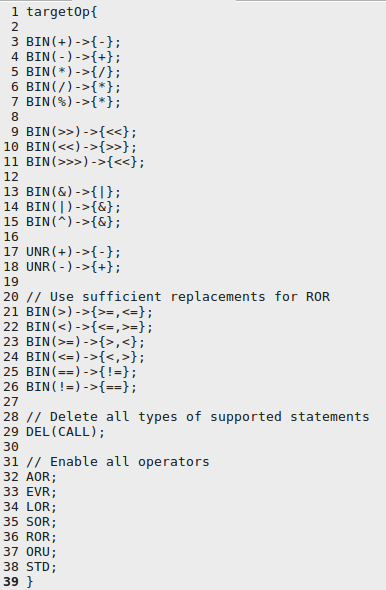
\includegraphics[width=.7\textwidth]{img/case_study/mml-used.png}
	\caption{پرونده‌ی mml ساخته شده جهت تولید جهش‌یافته‌ها}
	\label{fig:mml-used}
\end{figure}
\end{itemize}
 پس از انجام تحلیل جهش برای پرونده‌های حاوی خطا و سالم نتایج در جدول MutationMetrics قرار داده شد که نمایی از این جدول در شکل \ref{fig:mutation-metrics}  آمده است. 
 
 
 \begin{figure}[H]
 	\centering
 	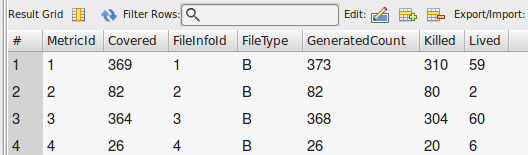
\includegraphics[width=.7\textwidth]{img/case_study/mutation-metrics.png}
 	\caption{نمایی از جدول نتایج تحلیل جهش}
 	\label{fig:mutation-metrics}
 \end{figure}
 